\documentclass[10pt,xcolor={usenames}]{beamer}
\usepackage{beamerthemesplit}
\usetheme{madrid}
%\usecolortheme{crane}

\usepackage[T2A]{fontenc}
%\usepackage[cp1251]{inputenc} %for Windows
\usepackage[utf8]{inputenc}

%\documentclass[a4paper, 1wpt]{amsart}
\usepackage[english]{babel}

\usepackage{cmap}
\usepackage{amsfonts, amssymb, amscd, amsmath}
\usepackage{latexsym}
\usepackage[matrix,arrow,curve]{xy}
\usepackage{mathabx}%,mathtools}
%\usepackage{color}

\usepackage{graphics}
\usepackage{graphicx}
 \usepackage{color}
 \usepackage{transparent}
%\usepackage[dvipsnames]{xcolor}

\usepackage{pbox}
\usepackage{tikz}
\usepackage{array}
%\usetikzlibrary{matrix,decorations.pathreplacing,positioning}
%\usepackage{scalerel}
\usepackage{hyperref}

\usepackage{parskip}
\usepackage{array}
\usepackage{epigraph}
\usepackage{animate}
\usepackage{stackrel}

%\DeclareSymbolFont{cyrillic}{T2A}{cmr}{m}{n}
%\DeclareMathSymbol{\Tse}{\mathalpha}{cyrillic}{214}


\newcolumntype{M}[1]{>{\centering\arraybackslash}m{#1}}

%\renewcommand{\contentsname}{GGGGGGGGGGGGG}

\definecolor{emph}{RGB}{200,90,0}

\newcolumntype{P}[1]{>{\centering\arraybackslash}p{#1}}

\newcommand*\circled[1]{\tikz[baseline=(char.base)]{
            \node[shape=circle,draw,inner sep=2pt] (char) {#1};}}

\DeclareMathOperator{\Cone}{Cone}
\DeclareMathOperator{\pt}{pt}
\DeclareMathOperator{\Ker}{Ker}
\DeclareMathOperator{\id}{id}
\DeclareMathOperator{\codim}{codim}
\DeclareMathOperator{\sgn}{sgn}
\DeclareMathOperator{\Imm}{Im}
\DeclareMathOperator{\im}{Im}
\DeclareMathOperator{\supp}{supp}
\DeclareMathOperator{\const}{const}
\DeclareMathOperator{\Hom}{Hom}
\DeclareMathOperator{\rk}{rk}
\DeclareMathOperator{\diag}{diag}
\DeclareMathOperator{\conv}{conv}
\DeclareMathOperator{\tr}{tr}
\DeclareMathOperator{\re}{Re}
\DeclareMathOperator{\PH}{PH}
\DeclareMathOperator{\EMST}{EMST}
\DeclareMathOperator{\LMST}{LMST}
\DeclareMathOperator{\Hilb}{P}
\DeclareMathOperator{\PD}{PD}

\DeclareMathOperator{\Sym}{Sym}

\DeclareMathOperator{\low}{low}

\DeclareMathOperator{\nc}{nc}


\DeclareMathOperator{\dist}{dist}
\DeclareMathOperator{\grad}{grad}

\newcommand{\ko}{\Bbbk}
\newcommand{\Fo}{\mathbb{F}}
\newcommand{\Zo}{\mathbb{Z}}
\newcommand{\Ro}{\mathbb{R}}
\newcommand{\Rg}{\mathbb{R}_{\geqslant 0}}
\newcommand{\Co}{\mathbb{C}}
\newcommand{\Qo}{\mathbb{Q}}
\newcommand{\Noo}{\mathbb{N}}
\newcommand{\Zt}{\Zo_2}
\newcommand{\Eo}{\mathbb{E}}

\newcommand{\br}{\widetilde{\beta}}
\newcommand{\eqd}{\stackrel{\text{\tiny def}}{=}}
\newcommand{\toiso}{\stackrel{\cong}{\to}}

\newcommand{\wh}[1]{{\widehat{#1}}}
\newcommand{\ca}[1]{\mathcal{#1}}

\newcommand{\Ch}{\check{C}}

\newcommand{\Hr}{\widetilde{H}}
\newcommand{\dd}{\partial}
\newcommand{\Ca}{\mathcal{C}}
\newcommand{\F}{\mathcal{F}}


\newcommand{\RP}{\mathbb{R}P}
\newcommand{\CP}{\mathbb{C}P}


\title[Topology intro]{Topological data analysis \\ Lecture 5}
\author[Anton Ayzenberg]{ Anton Ayzenberg }% \\  \texttt{ayzenberga@gmail.com}}
\date[FCS-YDS'24]{Spring 2024 \\ Faculty of Computer Science / Yandex Data School}
\institute[ATA \& Noeon Research]{ATA Lab, FCS NRU HSE \\ Noeon Research}

\begin{document}

\maketitle


\begin{frame}{Persistent homology: practical algorithm}

\begin{itemize}
  \item Previously we had $D_1,D_2,\ldots$ matrices of simplicial differentials $\dd_i\colon C_i(K)\to C_{i-1}(K)$
  \item $D_i$ is the incidence matrix between $i$-dim simplices and $(i-1)$-dim simplices at least over $\Zt$.
  \item Now we combine them all in a huge matrix $D$ of size $N\times N$,
  \item where $N$ is the total number of simplices in a filtration.
  \item The order of rows and columns as in the array Simplices.
\end{itemize}
\end{frame}

\begin{frame}{Gauss elimination on columns}

\begin{itemize}
  \item Reduce $D$ by elementary operations \textcolor{red}{on columns}.
  \item It is allowed to any column, \textcolor{blue}{to add another column multiplied by a scalar}.
  \item We move from left to right checking all $1\leqslant j \leqslant N$.
  \item Let $\low(j)$ denote \textcolor{red}{the index of the lowest nonzero element} in $j$-th column.
  \item For each $j$ we loop through $r<j$, and look for $r$ such that $\low(r)=\low(j)$.
  \item When we meet such $r$, we reduce $j$-th column by $r$-th column.
  \item We loop until $\low\colon[N]\to[N]$ becomes injective. This is called \textcolor{blue}{the reduced form of a matrix}.
  \item \textcolor{red}{Permutations are not allowed}.
\end{itemize}
\end{frame}

{
\setbeamercolor{background canvas}{bg=black!90}
%\setbeamercolor{title}{bg=black!90}
\setbeamercolor{frametitle}{bg=black}
%\setbeamercolor{normal text}{fg=green}


\begin{frame}{\textcolor{green}{\texttt{You have the Matrix...}}}
\small
\setlength{\arraycolsep}{3pt}
\medmuskip = 1mu % default: 4mu plus 2mu minus 4mu
%\ttfamily Some text

\[\color{green}
%\mathtt{
\begin{array}{c|ccccccccccccccc|}
& 1 & 2 & 3 & 4 & 23 & 34 & 12 & 24 & 234 & 13 & 14 & 123 & 124 & 134 & 1234\\
\hline
1   &&&&&{\transparent{0.6}0}&{\transparent{0.4}0}&{\transparent{0.8}1}&{\transparent{0.4}0}&&{\transparent{0.6}1}&{\transparent{0.4}1}&&&& \\
2   &&&&&{\transparent{0.8}1}&{\transparent{0.6}0}&{\circled{1}}&{\transparent{0.6}1}&&{\transparent{0.8}0}&{\transparent{0.6}0}&&&& \\
3   &&&&&{\transparent{1}\circled{1}}&{\transparent{0.8}1}&&{\transparent{0.8}0}&&\circled{1}&{\transparent{0.8}0}&&&& \\
4   &&&&&&{\circled{1}}&&\circled{1}&{\transparent{0.2}0}&&\circled{1}&&&& \\
23  &&&&&&&&&{\transparent{0.4}1}&&&{\transparent{0.2}1}&&&\\
34  &&&&&&&&&{\transparent{0.6}1}&&&{\transparent{0.4}0}&{\transparent{0.2}0}&{\transparent{0.2}1}& \\
12  &&&&&&&&&{\transparent{0.8}0}&&&{\transparent{0.6}1}&{\transparent{0.4}1}&{\transparent{0.4}0}& \\
24  &&&&&&&&&\circled{1}&&&{\transparent{0.8}0}&{\transparent{0.6}1}&{\transparent{0.6}0}& \\
234 &&&&&&&&&&&&{\transparent{0.9}0}&{\transparent{0.8}0}&{\transparent{0.8}0}&{\transparent{0.2}1} \\
13  &&&&&&&&&&&&\circled{1}&{\transparent{0.9}0}&{\transparent{0.9}1}&{\transparent{0.4}0} \\
14  &&{\transparent{0.2}0}&&&&&&&&{\transparent{0.2}0}&&&\circled{1}&\circled{1}&{\transparent{0.6}0} \\
123 &&{\transparent{0.4}0}&&&{\transparent{0.2}0}&&&&&{\transparent{0.4}0}&&&&&{\transparent{0.8}1} \\
124 &&{\transparent{0.6}0}&&{\transparent{0.2}0}&{\transparent{0.4}0}&&{\transparent{0.2}0}&&&{\transparent{0.6}0}&{\transparent{0.2}0}&&&&{\transparent{0.9}1} \\
134 &&{\transparent{0.8}0}&&{\transparent{0.4}0}&{\transparent{0.6}0}&&{\transparent{0.4}0}&&&{\transparent{0.8}0}&{\transparent{0.4}0}&&&&\circled{1} \\
1234&&{\transparent{0.9}0}&&{\transparent{0.6}0}&{\transparent{0.8}0}&&{\transparent{0.6}0}&&&{\transparent{0.9}0}&{\transparent{0.6}0}&&&& \\
\hline
\end{array}
%}
\]
\end{frame}


\begin{frame}{\textcolor{green}{\texttt{After Gauss elimination in columns}}}
\small
\setlength{\arraycolsep}{3pt}
\medmuskip = 1mu % default: 4mu plus 2mu minus 4mu

\[\color{green}
\begin{array}{c|ccccccccccccccc|}
& 1 & 2 & 3 & 4 & 23 & 34 & 12 & 24 & 234 & 13 & 14 & 123 & 124 & 134 & 1234\\
\hline
1   &&&&&&&1&&&&&&&& \\
2   &&&&&1&&\circled{1}&&&&&&&& \\
3   &&&&&\circled{1}&1&&&&&&&&& \\
4   &&&&&&\circled{1}&&&&&&&&& \\
23  &&&&&&&&&1&&&&&&\\
34  &&&&&&&&&1&&&&&& \\
12  &&&&&&&&&&&&1&1&& \\
24  &&&&&&&&&\circled{1}&&&&1&& \\
234 &&&&&&&&&&&&&&&1 \\
13  &&&&&&&&&&&&\circled{1}&&& \\
14  &&&&&&&&&&&&&\circled{1}&& \\
123 &&&&&&&&&&&&&&&1 \\
124 &&&&&&&&&&&&&&&1 \\
134 &&&&&&&&&&&&&&&\circled{1} \\
1234&&&&&&&&&&&&&&& \\
\hline
\end{array}
\]

\end{frame}
}

\begin{frame}{After Gauss}

Look at the reduced matrix $M$.

\begin{block}{Theorem}
\begin{itemize}
  \item Let $j=\low(s)\neq 0$ in $M$. Then \textbf{Simplices[j]} gives birth to homology of rank $\dim\mbox{Simplices[j]}$ and \textbf{Simplices[s]} kills this homology. Each such pair $(j,s)$ gives rise to \textcolor{red}{the interval module $I_{[BirthTimes[j],BirthTimes[s])}$}.
  \item If the whole $r$-th column vanish and moreover $r\notin\low([N])$, then Simplices[r] gives birth to homology of rank $\dim\mbox{Simplices[r]}$ which never dies. It gives \textcolor{red}{the interval module $I_{[BirthTimes[r],+\infty)}$}.
\end{itemize}
\textbf{Persistent homology} of the filtration is the direct sum of all the listed interval modules.
\end{block}

\end{frame}

\begin{frame}{Example}

\begin{center}
\includegraphics[scale=0.2]{pictures/filtration7.pdf}
\end{center}

\end{frame}

\begin{frame}{Our reduced matrix}
\footnotesize
\setlength{\arraycolsep}{2.5pt}
\medmuskip = 1mu % default: 4mu plus 2mu minus 4mu

\[
\begin{array}{c|ccccccccccccccc|}
& 1 & 2 & 3 & 4 & 23 & 34 & 12 & 24 & 234 & 13 & 14 & 123 & 124 & 134 & 1234\\
\hline
1   &&&&&&&1&&&&&&&& \\
2   &&&&&1&&\circled{1}&&&&&&&& \\
3   &&&&&\circled{1}&1&&&&&&&&& \\
4   &&&&&&\circled{1}&&&&&&&&& \\
23  &&&&&&&&&1&&&&&&\\
34  &&&&&&&&&1&&&&&& \\
12  &&&&&&&&&&&&1&1&& \\
24  &&&&&&&&&\circled{1}&&&&1&& \\
234 &&&&&&&&&&&&&&&1 \\
13  &&&&&&&&&&&&\circled{1}&&& \\
14  &&&&&&&&&&&&&\circled{1}&& \\
123 &&&&&&&&&&&&&&&1 \\
124 &&&&&&&&&&&&&&&1 \\
134 &&&&&&&&&&&&&&&\circled{1} \\
1234&&&&&&&&&&&&&&& \\
\hline
\end{array}
\]
\small
Circled elements have indices: $[3,23]$, $[4,34]$, $[2,12]$, $[24,234]$, $[13,123]$, $[14,124]$, $[134,1234]$.

\end{frame}



\begin{frame}{Reading births and deaths}

\begin{tabular}{M{4cm} p{8cm}}
\begin{center}
\includegraphics[scale=0.12]{pictures/norns.jpg} \break
{\footnotesize Norns determine the fate of homology}
\end{center}
  & \parbox{8cm}{ \begin{center}
                    \includegraphics[scale=0.08]{pictures/filtration7.pdf}
                  \end{center}
  %\hfill \break
  \begin{itemize}
                                                      \item We see pairs: $[3,23]$, $[4,34]$, $[2,12]$, $[24,234]$, $[13,123]$, $[14,124]$, $[134,1234]$.
                                                      \item For example, vertex $3$ gives rise to homology which dies when $23$ appears.
                                                      \item $3$ appears at time $0$, and $23$ --- at time $t_1$.
                                                      \item Hence we have interval module $I_{[0;t_1)}$ in 0-th homology.
                                                      \item etc...
                                                    \end{itemize} }\\
%  {\footnotesize Norns determine the fate of homology} & \\
\end{tabular}
We have decomposition: $I_{[0;t_1)}\oplus I_{[0;t_2)}\oplus I_{[0;t_3)}\oplus I_{[t_3;t_4)}\oplus I_{[t_5;t_7)}\oplus I_{[t_6;t_7)}$.

\end{frame}

\begin{frame}{Real times}

\begin{itemize}
  \item Let $K_t$, $t\in\Ro$ be a collection of simplicial complexes on vertex set $[m]$,
  \item such that $t_1<t_2$ implies $K_{t_1}\subseteq K_{t_2}$.
  \item This is called \textcolor{red}{a filtration with real time}.
  \item Changes may occur only at discrete time moments.
  \item Therefore, the only difference is that BirthTimes stores real values.
  \item The algorithm above outputs the interval decomposition.
\end{itemize}

\end{frame}

\begin{frame}{How to encode persistent homology?}

Persistence diagram instead of barcode.

\begin{center}
\includegraphics[scale=0.15]{pictures/persdiagram.pdf}
\end{center}

\end{frame}

\begin{frame}{Philosophy}

\begin{itemize}
  \item If some homology lives long, then it is \textbf{a meaningful homology}.
  \item The lifetime = death time - birth time.
  \item Lifetime is long, if the point of persistence diagram is far from the diagonal $y=x$.
  \item Points close to the diagonal are considered noise.
  \item Long-live-homology are important topological features of a filtration.
\end{itemize}

\end{frame}






\begin{frame}{Filtrations: \v{C}ech}

Demonstration: \href{https://play.unity.com/mg/other/builds-4z-1}{press to play in browser}
\pause

\begin{itemize}
  \item Let $X=\{x_1,\ldots,x_m\}\subset \Ro^d$ be a point-cloud.
  \item Let $X_t=\bigcup B_{t/2}(x_i)$.
  \item $X_t$ is a filtration, but not \textcolor{blue}{of simplicial complexes}.\pause
  \item Replace $X_t$ by its \textbf{nerve}!
\end{itemize}

\begin{block}{Nerve complex}
Let $K^{\check{C}}_t$ be a simplicial complex on $[m]$, such that $\{i_1,\ldots,i_s\}\in K^{\check{C}}_t$ iff
\[
B_{t/2}(x_{i_1})\cap\cdots\cap B_{t/2}(x_{i_s})\neq\varnothing
\]
\end{block}

\end{frame}

\begin{frame}{Nerve complex and Nerve theorem}

Let $K^{\check{C}}_t$ be a simplicial complex on $[m]$, such that $\{i_1,\ldots,i_s\}\in K^{\check{C}}_t$ iff $B_{t/2}(x_{i_1})\cap\cdots\cap B_{t/2}(x_{i_s})\neq\varnothing$.

\begin{block}{Nerve theorem}
\[
X_t\simeq K^{\check{C}}_t
\]
\end{block}

\pause
\begin{itemize}
  \item Therefore $X_t$ and $K^{\check{C}}_t$ have the same homology for each $t$.
  \item Hence they have the same persistent homology.
  \item We can work with simplicial filtration $\{K^{\check{C}}_t\}$ called \textbf{\v{C}ech filtration}. \pause
  \item Simplex $I$ is born at the time = minimal $t$ for which balls of radii $t/2$ around $x_i$, $i\in I$, intersect.\pause
  \item It may be \textcolor{red}{difficult to find this number} in practice.
\end{itemize}

\end{frame}

\begin{frame}{Vietoris--Rips filtration}

\begin{itemize}
  \item Let $X=\{x_1,\ldots,x_m\}\subset \Ro^d$ be a point-cloud.\pause
  \item $K^{VR}_t$ be a simplicial complex on $[m]$ such that
  \item $I\in K^{VR}_t$ iff all pairwise distances between $x_i$ and $x_j$, for $i\neq j$, $i,j\in I$, are less than $t$.
  \item Simplex $I$ is born at time moment \textcolor{red}{$\max_{i\neq j\in I}\dist(x_i,x_j)$}.\pause
  \item $\{K^{VR}_t\}$ is called \textbf{Vietoris--Rips filtration}.\pause
  \item Very \textcolor{blue}{easy to compute birth times}!\pause
  \item Can be adapted to  \textcolor{red}{any finite metric space}, e.g. metric graph.
\end{itemize}

\end{frame}

%\begin{frame}{Some experiments with Dionysus2}
%
%\href{https://colab.research.google.com/drive/146yQdZBsPGfYZwi1AGKJwSE5wjRwPnc1?usp=sharing}{Link to Google Colab}
%
%\begin{center}
%\includegraphics[scale = 0.2]{pictures/pythonComb.png}
%\end{center}
%
%\end{frame}



\begin{frame}{How to compare filtrations and diagrams?}

\begin{itemize}
  \item We have two filtrations $\{K_t\}$ and $\{L_t\}$ on the same set $[m]$.
  \item Set $\dist(\{K_t\},\{L_t\})=\max_{I\subset [m]}|\mbox{BirthTime}_K[I]-\mbox{BirthTime}_L[I]|$.\pause
  \item If $X=\{x_1,\ldots,x_m\}$ and $Y=\{y_1,\ldots,y_m\}$ are two data clouds and
  \item $\dist(X,Y)=\max_i\dist(x_i,y_i)$, and
  \item $K^{VR}_t$ and $L^{VR}_t$ are their Vietoris--Rips filtrations\pause, then
  \item \textbf{Exercise:} $\dist(\{K^{VR}_t\},\{L^{VR}_t\})\leqslant 2\dist(X,Y)$.\pause
  \item What about their persistent diagrams?
\end{itemize}

\end{frame}

\begin{frame}{Metric on diagrams}

Bottleneck distance (or Wasserstein, or Kantorovich metric)

\begin{center}
\includegraphics[scale = 0.4]{pictures/bottleneck.png}\break
Fig.from \href{https://gudhi.inria.fr/doc/latest/group\_\_bottleneck\_\_distance.html}{GUDHI Library}
\end{center}
\pause
\begin{block}{Stability theorem}
\[
\dist(\PD(\{K_t\}),\PD(\{L_t\}))\leqslant \dist(\{K_t\},\{L_t\}).
\]
\end{block}

\end{frame}

\begin{frame}{Generalizations of persistent modules}

We can hardly see this slide. However if we do, then it is time to switch to whiteboard

\end{frame}


%\setbeamercolor{background canvas}{bg=white}
%\setbeamercolor{title}{bg=black}
%\setbeamercolor{frametitle}{bg=Blue}

\begin{frame}{Sources}

\begin{thebibliography}{12}

\bibitem{Baran} S.\,Barannikov, \textit{Framed Morse complex and its invariants}, Advances in Soviet Mathematics. Vol.21 (1994), pp. 93--115.

\bibitem{Che} H.\,Y.\,Cheung, T.\,C.\,Kwok, L.\,C.\,Lau, \textit{Fast matrix rank algorithms and applications}, J. ACM 60:5 (2013), Article 31.

\bibitem{EH} H.\,Edelsbrunner, J.\,L.\,Harer, Computational Topology: An Introduction, 2010.

\bibitem{MorozD} Morozov, Dionysus2 library \href{https://mrzv.org/software/dionysus2/}{https://mrzv.org/software/dionysus2/}

\bibitem{Zom} A.\,J.\,Zomorodian, Topology for computing, 2005.

\end{thebibliography}

\end{frame}

%
%
%\begin{frame}{Technical slide}
%\href{https://colab.research.google.com/drive/146yQdZBsPGfYZwi1AGKJwSE5wjRwPnc1?usp=sharing}{Colab}
%
%\href{https://play.unity.com/mg/other/builds-4z-1}{Unity}
%
%\begin{center}
%\animategraphics[controls,scale=0.25]{5}{pictures/Simplify/Simplify_}{0}{1}
%\end{center}
%\end{frame}


\end{document} 